\documentclass{jarticle}

\usepackage[dvipdfmx]{graphicx}
\usepackage{float}
\usepackage{url}

\title{放射線の計測}
\author{2511198 肥田幸久 \\ 共同実験者 \\ }
\date{2025年10月10日作成}

\begin{document}
\maketitle



\section{実験の目的}

GM計数管を用いて, 放射性原子の放射性崩壊の法則と物質による放射線の吸収について調べる.



\section{実験の原理}


\subsection{放射性原子の崩壊}

原子核は陽子と中性子から構成されているが, 原子核の質量は, 陽子と中性子の質量の和よりも小さく, この質量の差を質量欠損という.
これは, 原子核を構成する陽子と中性子が結合しているためであり, 質量欠損$\Delta m$ に相当するエネルギー$\Delta mc^2$を結合エネルギーという.

ある原子核が安定でない場合, その原子核は放射性崩壊を起こし, より安定な原子核に変化する.
このとき, $\alpha$線, $\beta$線, $\gamma$線などの放射線が放出される.
この現象が放射性原子の崩壊である.


\subsection{放射性崩壊の計数値の分布}

放射性原子の崩壊は, ある一定の確率で起こる現象であり, 個々の原子については, いつ崩壊するかを予測することはできない.
放射性原子が崩壊する確率は, その原子核の種類に依存する.

ある核種$\mathrm{A}$が時刻$t$において$\mathcal{N}$個あるとする.
微小時間$\mathrm{d}t$の間に崩壊を起こして他の核種$\mathrm{B}$に変化する数を$\mathrm{d}N$とすると, 単位時間あたりの崩壊数$\mathrm{d}\mathcal{N}/\mathrm{d}t$は$\mathcal{N}$に比例し, 比例定数(崩壊定数)を$\lambda$とすると, 次のように表される.
\begin{equation}
  \frac{\mathrm{d}\mathcal{N}}{\mathrm{d}t} = -\lambda \mathcal{N}
\end{equation}

時刻$t=0$における核種$\mathrm{A}$の数を$\mathcal{N}_0$とすると, 時刻$t$における核種$\mathrm{A}$の数は平均的に次のようになる.
\begin{equation}
  \mathcal{N}(t) = \mathcal{N}_0 e^{-\lambda t}
\end{equation}
また, この数が半分になる時間を半減期$\tau$といい, 次の関係が成り立つ.
\begin{equation}
  \tau = (\log_e 2)/\lambda
  = 0.693/\lambda
\end{equation}

次に, $\lambda t$が$1$に比べて十分小さいとき, $e^{-\lambda t}$はテイラー展開により,
\begin{equation}
  e^{-\lambda t} \cong 1 - \lambda t
\end{equation}
と近似できる.
したがって, 時刻$t$における核種$\mathrm{A}$の数は次のように表される.
\begin{equation}
  \mathcal{N}(t)=\mathcal{N}_0-\mathcal{N}_0\lambda t
\end{equation}
この式から, 放射性崩壊の数を時間$t$にわたって観測して得られる計数値$N$の平均値$\overline{N}$は
\begin{equation}
  \overline{N} = \mathcal{N}_0\lambda t
\end{equation}
と期待できる.

そしてその計数値$N$の確率$P(N)$は, 次のポアソン分布に従う.
\begin{equation}
  P(N) = \frac{(\overline{N})^N}{N!}e^{-\overline{N}}, \quad
  \sum_{N=0}^{\infty} P(N) = 1
  \label{eq:poisson}
\end{equation}
また, 平均値$\overline{N}$が大きくなると, ポアソン分布は次のガウス分布(正規分布)に近づく.
\begin{equation}
  G(N) = \frac{1}{\sqrt{2\pi\overline{N}}} \exp \left\{-\frac{(N-\overline{N})^2}{2\overline{N}}\right\}
\end{equation}


\subsection{$\beta$線の吸収}

$\beta$線が物質中を通過するとき, 物質中の原子と相互作用してエネルギーを失い, 次第に減衰していく.
このとき$\beta$線の電子$\mathcal{N}$個が物質を通過する間に吸収されて減衰する割合は, その物質の厚さ$\mathrm{d}x$に比例し, 比例定数(線吸収係数)を$\mu$とすると, 次のように表される.
\begin{equation}
  \frac{\mathrm{d}\mathcal{N}}{\mathrm{d}x} = -\mu \mathcal{N}
\end{equation}
物質に入射前における電子の数を$\mathcal{N}_0$とすると, 物質の厚さ$x$を通過した後に残っている電子の数は次のようになる.
\begin{equation}
  \mathcal{N}(x) = \mathcal{N}_0 e^{-\mu x}
\end{equation}
また, 物質を通過して出てくる電子数は一般に, 物質層の厚さ$x$の代わりに単位面積あたりの質量$\rho_s$($\rho_s=\rho x$, ただし$\rho$は密度)を, 線吸収係数$\mu$の代わりに質量吸収係数$\mu_m$($\mu_m=\mu/\rho$)を用いて次のように表される.
\begin{equation}
  \mathcal{N}(x) = \mathcal{N}_0 e^{-\mu_m \rho_s}
\end{equation}



\section{実験方法}


本実験では, 図\ref{fg:radiation-method}のような装置を用いて, 放射線の計測を行った.
印加電圧は$500\ \mathrm{V}$に設定し, GM計数管の下段に$\beta$線源($^{137}_{55}\mathrm{Cs}$)を, 上段に吸収板を挟んで計測した.

\begin{figure}[H]
  \begin{center}
    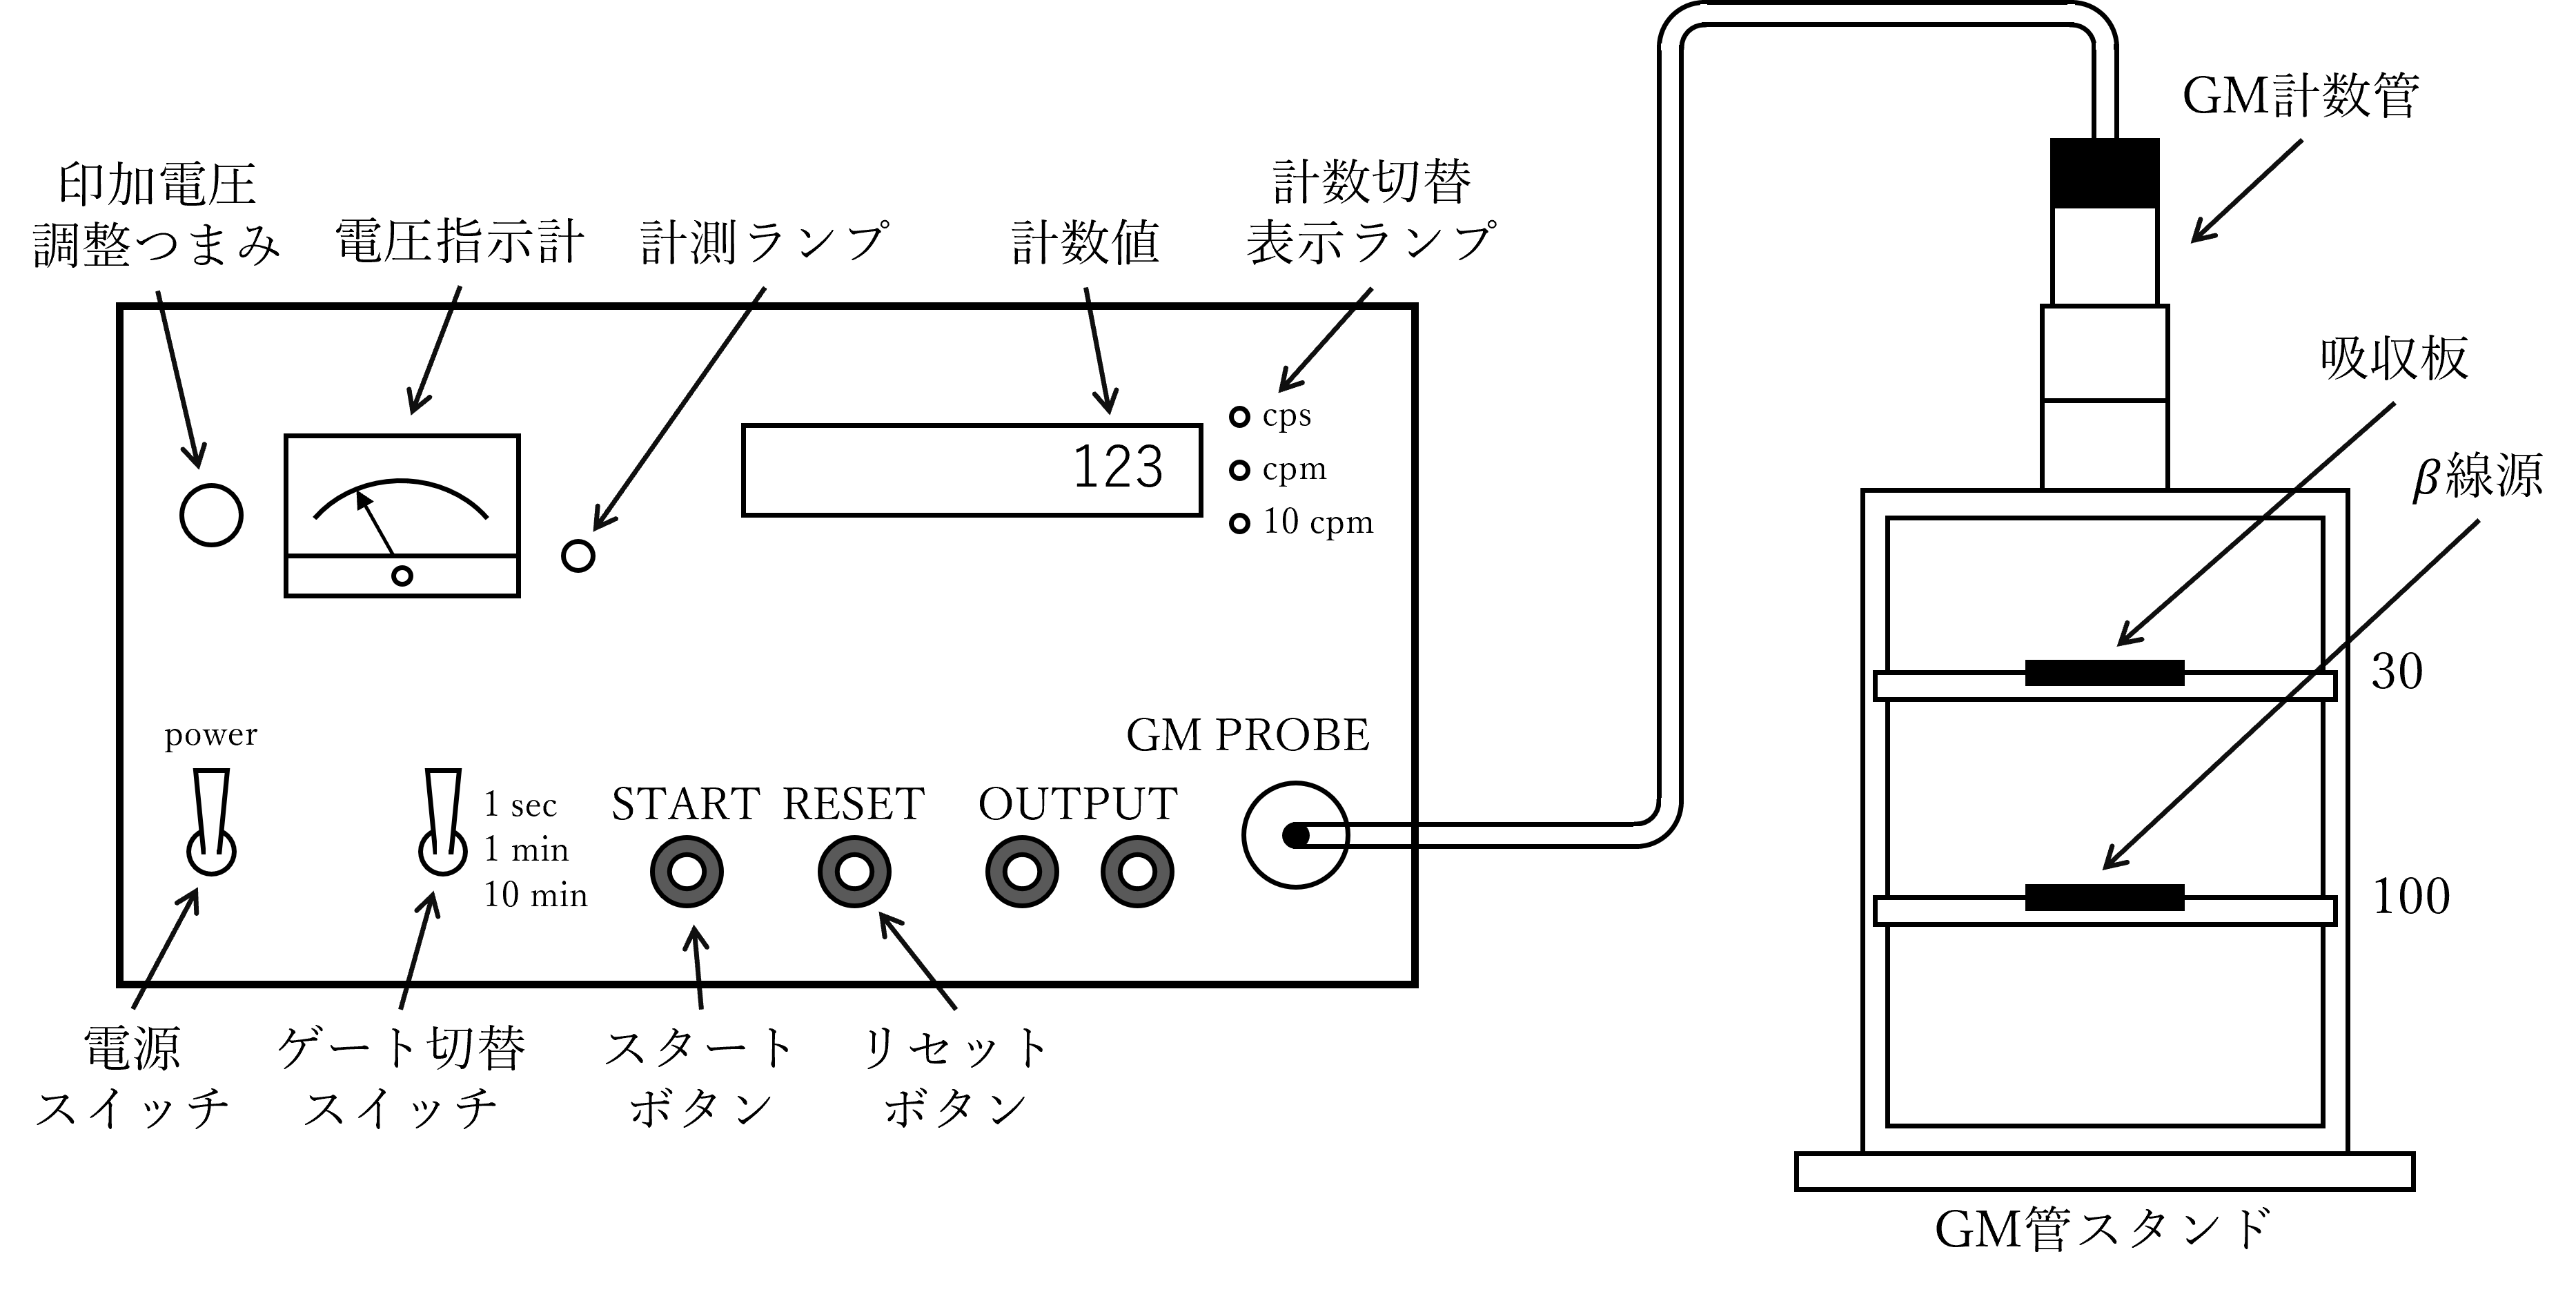
\includegraphics[width=110mm]{experimental_equipment.png}
    \caption{放射線の計測の実験装置}
    \label{fg:radiation-method}
  \end{center}
\end{figure}


\subsection{自然計数の測定}

$\beta$線源を実験台に持ってこない状態で, 計数時間を$60\ \mathrm{s}$として, 自然計数を$20$回測定した.


\subsection{$\beta$線の計数値の分布の観測}

$\beta$線源のみをGM計数管の下段に入れ, 計数時間を$1\ \mathrm{s}$として, $\beta$線の計数値を測定した.
この測定を$\beta$線源を入れる位置を変えてそれぞれ$300$回以上測定を行った.


\subsection{$\beta$線の吸収の測定}

本実験で使用する$\beta$線源は$\gamma$線も放出するため, 初めに, 厚さ約$1\ \mathrm{mm}$の$\mathrm{Al}$板で遮蔽することで, $\beta$線のみを計測した.

次に, $\beta$線の吸収を調べるため, $\mathrm{Cu}$および$\mathrm{Ti}$の薄板をそれぞれ$0$枚から$6$枚まで$1$枚ずつ増やすことで, 吸収板の厚さを変化させ測定した.



\section{実験結果}


\subsection{自然計数の測定}

\begin{table}[H]
  \begin{minipage}[t]{0.45\textwidth}
    \centering
    \caption{自然計数の測定}
    \label{tb:natural-count}
    \begin{tabular}{cc}
      \hline
      回数 & 計数値$\mathcal{N}$ \\
      \hline
      1 & 15 \\
      2 & 16 \\
      3 & 14 \\
      4 & 16 \\
      5 & 16 \\
      6 & 14 \\
      7 & 11 \\
      8 & 12 \\
      9 & 13 \\
      10 & 17 \\
      11 & 16 \\
      12 & 19 \\
      13 & 16 \\
      14 & 21 \\
      15 & 7 \\
      16 & 19 \\
      17 & 23 \\
      18 & 16 \\
      19 & 16 \\
      20 & 14 \\
      \hline
    \end{tabular}
  \end{minipage}
  \begin{minipage}[t]{0.45\textwidth}
    \centering
    \caption{計数値$\mathcal{N}$と出現回数$\mathrm{n}$}
    \label{tb:count-distribution}
    \begin{tabular}{cc}
      \hline
      計数値$\mathcal{N}$ & 出現回数$\mathrm{n}$ \\
      \hline
      7 & 1 \\
      8 & 0 \\
      9 & 0 \\
      10 & 0 \\
      11 & 1 \\
      12 & 1 \\
      13 & 1 \\
      14 & 3 \\
      15 & 1 \\
      16 & 6 \\
      17 & 1 \\
      18 & 0 \\
      19 & 3 \\
      20 & 0 \\
      21 & 1 \\
      23 & 1 \\
      \hline
    \end{tabular}
  \end{minipage}
\end{table}

これより最頻値は$16$, 中央値は$16$, 平均値$N_0$は$15.65$と求まった.


\subsection{$\beta$線の計数値の分布の観測}

ポアソン分布$P(N)$は式(\ref{eq:poisson})を用いて, また平均値$\overline{N}$と標準偏差$\sigma$は次の式を用いて求める.
\begin{equation}
  \overline{N} = \frac{\sum n_N N}{\sum n_N}
\end{equation}
\begin{equation}
  \sigma = \sqrt{\frac{\sum n_N (N-\overline{N})^2}{(\sum n_N) - 1}}
\end{equation}


\subsubsection{計測回数$100$回, 線源の位置$100\ \mathrm{mm}$の場合}

以下に, 計測回数$100$回, 計数時間$1\ \mathrm{s}$, 線源の位置$100\ \mathrm{mm}$の場合の計数値の分布の実験結果を示す.

\begin{table}[H]
  \centering
  \caption{計数値の分布の実験結果}
  \label{tb:count-distribution-100mm-100times}
  \begin{tabular}{cccccc}
    \hline
    計数値 & 出現回数 & 出現確率 & $N$と$n_N$の積 & 2乗偏差と$n_N$の積 & ポアソン分布 \\
    $N$ & $n_N$ & $n_N/\sum n_N$ & $n_N N$ & $n_N(N-\overline{N})^2$ & $P(N)$ \\
    \hline
    0 & 2 & 0.02 & 0 & 22.0448 & 0.03615283 \\
    1 & 8 & 0.08 & 8 & 43.0592 & 0.12002740 \\
    2 & 29 & 0.29 & 58 & 50.5296 & 0.19924549 \\
    3 & 20 & 0.20 & 60 & 2.0480 & 0.22049834 \\
    4 & 23 & 0.23 & 92 & 10.6352 & 0.18301362 \\
    5 & 6 & 0.06 & 30 & 16.9344 & 0.12152104 \\
    6 & 6 & 0.06 & 36 & 43.0944 & 0.06724164 \\
    7 & 2 & 0.02 & 14 & 27.0848 & 0.03189175 \\
    8 & 2 & 0.02 & 16 & 43.8048 & 0.01323508 \\
    9 & 2 & 0.02 & 18 & 64.5248 & 0.00488227 \\
    \hline
    合計 & 100 & 1 & 332 & 323.76 & \\
    \hline
  \end{tabular}
\end{table}


\subsubsection{計測回数$300$回, 線源の位置$100\ \mathrm{mm}$の場合}

以下に, 計測回数$300$回, 計数時間$1\ \mathrm{s}$, 線源の位置$100\ \mathrm{mm}$の場合の計数値の分布の実験結果を示す.

\begin{table}[H]
  \centering
  \caption{計数値の分布の実験結果}
  \label{tb:count-distribution-100mm-300times}
  \begin{tabular}{cccccc}
    \hline
    計数値 & 出現回数 & 出現確率 & $N$と$n_N$の積 & 2乗偏差と$n_N$の積 & ポアソン分布 \\
    $N$ & $n_N$ & $n_N/\sum n_N$ & $n_N N$ & $n_N(N-\overline{N})^2$ & $P(N)$ \\
    \hline
    0 & 8 & 0.02667 & 0 & 87.2961 & 0.03676043 \\
    1 & 40 & 0.13333 & 40 & 212.2138 & 0.03676043 \\
    2 & 54 & 0.18 & 108 & 91.7286 & 0.20056510 \\
    3 & 60 & 0.2 & 180 & 5.5207 & 0.22084446 \\
    4 & 72 & 0.24 & 288 & 34.9448 & 0.18238072 \\
    5 & 37 & 0.12333 & 185 & 106.5111 & 0.12049286 \\
    6 & 16 & 0.05333 & 96 & 116.3522 & 0.06633801 \\
    7 & 10 & 0.03333 & 70 & 136.6534 & 0.03130522 \\
    8 & 3 & 0.01 & 24 & 66.1760 & 0.01292645 \\
    \hline
    合計 & 100 & 1 & 991 & 857.3967 & \\
    \hline
  \end{tabular}
\end{table}


\subsubsection{計測回数$300$回, 線源の位置$60\ \mathrm{mm}$の場合}

以下に, 計測回数$300$回, 計数時間$1\ \mathrm{s}$, 線源の位置$60\ \mathrm{mm}$の場合の計数値の分布の実験結果を示す.

\begin{table}[H]
  \centering
  \caption{計数値の分布の実験結果}
  \label{tb:count-distribution-60mm-300times}
  \begin{tabular}{cccccc}
    \hline
    計数値 & 出現回数 & 出現確率 & $N$と$n_N$の積 & 2乗偏差と$n_N$の積 & ポアソン分布 \\
    $N$ & $n_N$ & $n_N/\sum n_N$ & $n_N N$ & $n_N(N-\overline{N})^2$ & $P(N)$ \\
    \hline
    1 & 1 & 0.00333 & 1 & 60.0108 & 0.00139064 \\
    2 & 1 & 0.00333 & 2 & 45.5175 & 0.00608172 \\
    3 & 1 & 0.00333 & 3 & 33.0242 & 0.01773158 \\
    4 & 15 & 0.05000 & 60 & 337.9627 & 0.03877305 \\
    5 & 22 & 0.07333 & 110 & 308.8252 & 0.06782699 \\
    6 & 33 & 0.11000 & 198 & 248.9579 & 0.09887668 \\
    7 & 29 & 0.09667 & 203 & 88.4745 & 0.12354877 \\
    8 & 39 & 0.13000 & 312 & 21.7429 & 0.13507999 \\
    9 & 42 & 0.14000 & 378 & 2.6955 & 0.13127774 \\
    10 & 34 & 0.11333 & 340 & 53.4087 & 0.11482426 \\
    11 & 37 & 0.12333 & 407 & 187.8679 & 0.09130269 \\
    12 & 19 & 0.06333 & 228 & 201.0994 & 0.06654951 \\
    13 & 13 & 0.04333 & 169 & 235.1810 & 0.04477588 \\
    14 & 4 & 0.01333 & 56 & 110.3900 & 0.02797426 \\
    15 & 6 & 0.02000 & 90 & 234.6251 & 0.01631210 \\
    16 & 2 & 0.00667 & 32 & 105.2217 & 0.00891728 \\
    17 & 1 & 0.00333 & 17 & 68.1175 & 0.00458803 \\
    18 & 1 & 0.00333 & 18 & 85.6242 & 0.00222944 \\
    \hline
    合計 & 300 & 1 & 2624 & 2428.7467 & \\
    \hline
  \end{tabular}
\end{table}


\subsubsection{計測回数$300$回, 線源の位置$30\ \mathrm{mm}$の場合}

以下に, 計測回数$300$回, 計数時間$1\ \mathrm{s}$, 線源の位置$30\ \mathrm{mm}$の場合の計数値の分布の実験結果を示す.

\begin{table}[H]
  \centering
  \caption{計数値の分布の実験結果}
  \label{tb:count-distribution-30mm-300times}
  \begin{tabular}{cccccc}
    \hline
    計数値 & 出現回数 & 出現確率 & $N$と$n_N$の積 & 2乗偏差と$n_N$の積 & ポアソン分布 \\
    $N$ & $n_N$ & $n_N/\sum n_N$ & $n_N N$ & $n_N(N-\overline{N})^2$ & $P(N)$ \\
    \hline
    20 & 2 & 0.00667 & 40 & 358.5842 & 0.00382690 \\
    21 & 3 & 0.01000 & 63 & 460.5363 & 0.00611657 \\
    22 & 3 & 0.01000 & 66 & 389.1963 & 0.00928329 \\
    23 & 5 & 0.01667 & 115 & 539.7605 & 0.01347691 \\
    24 & 12 & 0.04000 & 288 & 1058.0650 & 0.01874976 \\
    25 & 8 & 0.02667 & 200 & 563.1368 & 0.02504218 \\
    26 & 7 & 0.02333 & 182 & 382.2847 & 0.03215993 \\
    27 & 11 & 0.03667 & 297 & 449.1531 & 0.03977112 \\
    28 & 9 & 0.03000 & 252 & 261.4689 & 0.04742706 \\
    29 & 18 & 0.06000 & 522 & 346.8978 & 0.05460653 \\
    30 & 16 & 0.05333 & 480 & 183.8736 & 0.06077707 \\
    31 & 29 & 0.09667 & 899 & 165.6509 & 0.06546278 \\
    32 & 14 & 0.04667 & 448 & 27.0494 & 0.06830632 \\
    33 & 18 & 0.06000 & 594 & 2.7378 & 0.06911358 \\
    34 & 17 & 0.05667 & 578 & 6.3257 & 0.06787360 \\
    35 & 20 & 0.06667 & 700 & 51.8420 & 0.06475142 \\
    36 & 24 & 0.08000 & 864 & 163.4904 & 0.06005694 \\
    37 & 16 & 0.05333 & 592 & 208.5136 & 0.05419733 \\
    38 & 10 & 0.03333 & 380 & 212.5210 & 0.04762234 \\
    39 & 14 & 0.04667 & 546 & 440.6094 & 0.04077205 \\
    40 & 8 & 0.02667 & 320 & 349.5368 & 0.03403447 \\
    41 & 7 & 0.02333 & 287 & 405.3847 & 0.02771734 \\
    42 & 9 & 0.03000 & 378 & 667.1889 & 0.02203528 \\
    43 & 4 & 0.01333 & 172 & 369.4084 & 0.01711065 \\
    44 & 4 & 0.01333 & 176 & 450.2884 & 0.01298465 \\
    45 & 1 & 0.00333 & 45 & 134.7921 & 0.00963461 \\
    46 & 3 & 0.01000 & 138 & 477.0363 & 0.00699347 \\
    47 & 1 & 0.00333 & 47 & 185.2321 & 0.00496834 \\
    48 & 1 & 0.00333 & 48 & 213.4521 & 0.00345610 \\
    49 & 2 & 0.00667 & 98 & 487.3442 & 0.00235509 \\
    50 & 2 & 0.00667 & 100 & 551.7842 & 0.00157273 \\
    51 & 2 & 0.00667 & 102 & 620.2242 & 0.00102967 \\
    \hline
    合計 & 300 & 1 & 10017 & 11183.3700 & \\
    \end{tabular}
\end{table}


\subsection{$\beta$線の吸収の測定}


\subsubsection{$\gamma$線の計数値の測定}





\section{考察}





\begin{thebibliography}{99}

  \bibitem{ref1} 参考文献1の情報
  \bibitem{ref2} 参考文献2の情報
  \bibitem{ref3} 参考文献3の情報

\end{thebibliography}

\end{document}